\documentclass[../main.tex]{subfiles}
\begin{document}

This report is presenting two approaches to Optical Character Recognition (OCR). The approaches applied are k-Nearest Neighbor Classifier and Support Vector Machines. A general overview of the implementation is shown in \autoref{fig:model}. The data is loaded from the Char74k-Lite dataset and diveded, at random, into two databases. 80 \% is selected as the training set, and 20 \% is the test set. The data is then preprocessed, as described in \autoref{sec:fe}. A model is trained on the training set, before the model is passed to the classifier. The classifier is described in \autoref{sec:class}. The system output is the classifier error, which is given by
\begin{equation}
	E = \frac{N_{\rm fail}}{N_{\rm test}}
\end{equation}
where $N_{\rm fail}$ is the number of wrong classifications in the test set and $N_{\rm test}$ is the total number of samples in the test set.

\subsection{How to run the system}

\begin{figure}
  \centering
  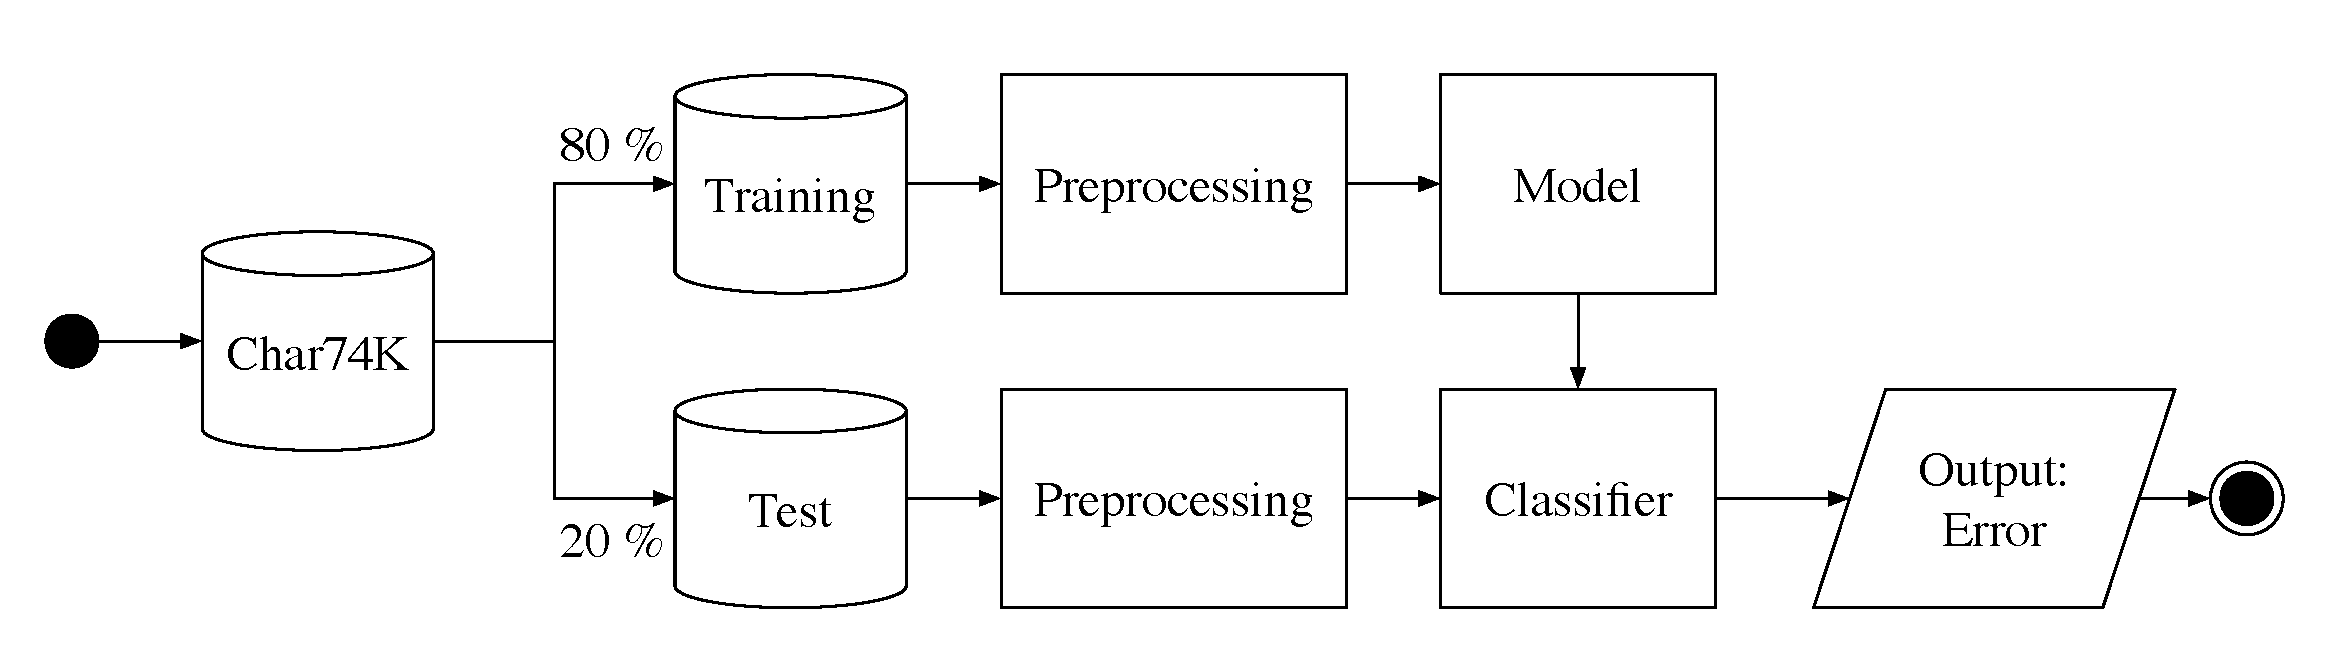
\includegraphics[width=\textwidth]{figures/model.eps}
  \caption{Model of OCR system.} 
  \label{fig:model}
\end{figure}

\end{document}